\documentclass[12pt,letterpaper]{article}
\usepackage{lipsum}
\usepackage{amssymb}
\usepackage{amsmath}
\usepackage{graphicx}
\graphicspath{ {} }
\usepackage{authblk}
\usepackage[top=0.8in, bottom= 0.8in, left= 0.8in, right= 0.8in]{geometry}
\usepackage{fancyhdr}

\pagestyle{fancy}
\begin{document}

%title and author details
\title{Laboratory III, Problem I: Electrical \\and Mechanical Energy}
\author[]{Cole Nielsen}
\date{}
\affil[]{Physic 1302W TA: Santosh Adhikari}
\pdfpagewidth 8.5in
\pdfpageheight 11in
%
%
\maketitle
\abstract{The conversion of electrical energy into mechanical energy was investigated using a capacitor connected to a motor that lifted a small mass . The energy transfer was considered in terms of vertical displacement of the mass when the motor was connected to the capacitor. In particular, it was determined that the height the mass is displaced is dependent quadratically on the capacitance of the capacitor used. The predicted equation for this relationship is as follows:\\
\begin{equation}
\Delta h (C) = 18.80C^2 + 1.262\times10^{-2}C -5.000\times10^{-5}
\end{equation}  }

\section{Introduction}
The scenario shown in \textit{Figure 1} was considered. In this scenario, a motor with a spool is attached to the top of a pole. A string attached to the spool also connects to a hanging mass $m$. A capacitor of capacitance $C$ is charged up to a fixed voltage $V_0$ using a power supply, and then is connected to the motor and is allowed to discharge. The capacitor discharging causes the motor's rotor to turn, lifting the mass by a height $\Delta h$, converting some of the electrical energy stored by the capacitor into mechanical energy. The rest of the energy is lost as heat. The relationship between the max displacement of the mass and the initial condition for the capacitance C is unknown, therefore this experiment seeks to determine this relationship.
\newline
\begin{center}
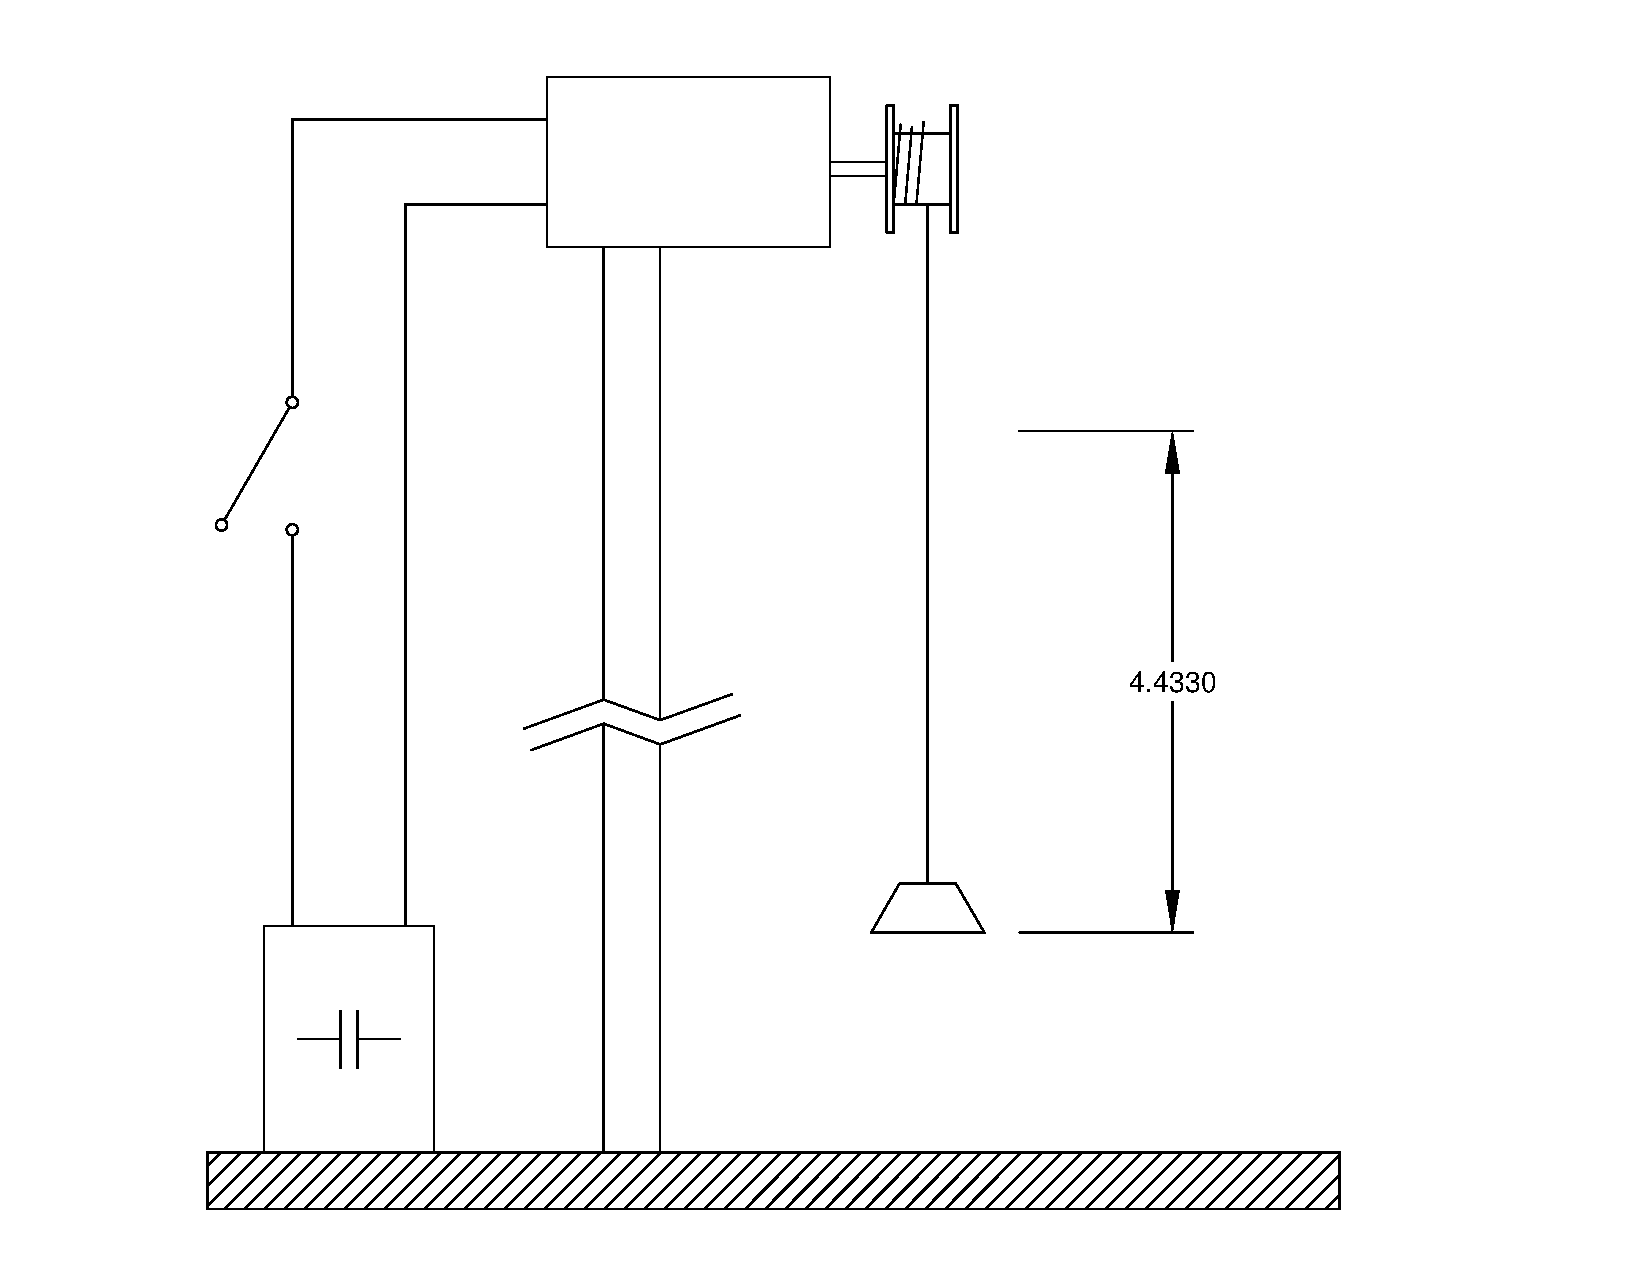
\includegraphics[scale=0.17]{physics_2_lab_2.png}
\\\textbf{Figure 1.} The experimental setup.
\end{center}%
\pagebreak
\section{Prediction}
To determine the displacement $\Delta h$ as a function of $C$, the function for the capacitive discharge in terms of current through the motor will be derived. This function will then be used to determine the acceleration of the mass as a function of time due to force on exerted on it by the motor. Knowing the acceleration as a function of time, the function for position ($\Delta h$) can be determined by integrating twice. The maximum $\Delta h$ of this function for several values of $C$ will be determined, and then plotted as a graph of of $\Delta h$ vs capacitance. Using computer based regression, a line of best fit will be found for $\Delta h(C)$ on this plot.\\\\
To perform this derivation, a few basic principles must be understood. The first of which is the operation of DC motors. DC motors are built with a rotor with magnetic coils wrapped around it. The rotor is then placed between two permanent magnets that produce a static magnetic field. When a current is applied to the rotor's coils, a field proportional to the current is generated by the coil. Magnetic attraction due to the static field and the coil's field then imparts a torque on the rotor which causes it to rotate. Since the field is proportional to the current, the attraction due to magnetism and the resulting torque is also proportional to current. This relationship implies that a motor with a certain amount of current flowing through it can only provide a limited amount of torque. The maximum value of this torque as called the stall torque (corresponding to a stall current). The next thing that must be understand is that DC motors have resistance in their windings, which results in a fairly significant loss of energy as heat when powered. This resistance will be generalized as $R$ initially.\\\\
The capacitive discharge of a resistor and capacitor circuit can be used to model the current as a function of time through the motor. The differential equation for RC discharge is given by $I'R + \frac{1}{c}I = 0$. The general solution for this differential equation is as follows, where $I_0$ is the initial current, which can be calculated using Ohm's law, the motor's resistance $R$ and the initial voltage of the capacitor $V_0$.

\begin{equation}
I(t)=I_0e^\frac{-t}{RC}=\frac{V_0}{R}e^\frac{-t}{RC}
\end{equation}
The force on the mass due to the motor can now be determined knowing this function. It is known torque is proportional to current for a motor, and force is proportional to torque for a fixed radius $r$. Since a fixed radius spool is used on the motor to wind up the string, it can be said the force exerted on the mass by the motor will be proportional to current. This proportionality can be used to produce an equation for $F(t)$:
\begin{equation}
I_0e^\frac{-t}{RC}=I(t)\propto F(t) = F_0e^\frac{-t}{RC}
\end{equation}
$F_0$ is simply the force that it takes to stall the motor at a given voltage (and the according stall current). Divide this equation by mass to get acceleration as a function of time, and then add acceleration due to gravity to get net acceleration:

\begin{equation}
a(t)=\frac{F(t)}{m}=\frac{F_0}{m}e^\frac{-t}{RC} \hspace{0.2in}\Rightarrow\hspace{0.2in} a_{net}(t) = \frac{F_0}{m}e^\frac{-t}{RC} + g
\end{equation}
Integrate this twice to get the position function for $\Delta h$. The initial velocity and position are zero.
\begin{equation}
\Delta h(t) = \frac{1}{2}gt^2 + \frac{F_0}{m}R^2C^2e^\frac{-t}{RC} + \frac{F_0}{m}RCt-\frac{F_0}{m}R^2C^2
\end{equation}
It is difficult to find the maximum value of this function explicitly, so to produce a predicted plot of $\Delta h$ for this problem, several values for C in the range of the capacitors used will plugged in and the maxima determined, and then plotted. To fit the range of capacitors used in the experiment, capacitances in the range [0,0.4] Farad will be used in 50 mF intervals. The value for $\frac{F_0}{m}$ will also be 19.1, and $R$ will be 2.6 $\Omega$. These values will be determined in later sections. Below in \textit{Figure 2} is the approximate plot for the predicted $\Delta h(t)$.
\begin {figure}[htb!]
  \begin{center}
    	\resizebox{0.49\textwidth}{!}{% GNUPLOT: LaTeX picture
\setlength{\unitlength}{0.240900pt}
\ifx\plotpoint\undefined\newsavebox{\plotpoint}\fi
\sbox{\plotpoint}{\rule[-0.200pt]{0.400pt}{0.400pt}}%
\begin{picture}(1500,900)(0,0)
\sbox{\plotpoint}{\rule[-0.200pt]{0.400pt}{0.400pt}}%
\put(171.0,131.0){\rule[-0.200pt]{4.818pt}{0.400pt}}
\put(151,131){\makebox(0,0)[r]{ 0}}
\put(1419.0,131.0){\rule[-0.200pt]{4.818pt}{0.400pt}}
\put(171.0,260.0){\rule[-0.200pt]{4.818pt}{0.400pt}}
\put(151,260){\makebox(0,0)[r]{ 0.5}}
\put(1419.0,260.0){\rule[-0.200pt]{4.818pt}{0.400pt}}
\put(171.0,389.0){\rule[-0.200pt]{4.818pt}{0.400pt}}
\put(151,389){\makebox(0,0)[r]{ 1}}
\put(1419.0,389.0){\rule[-0.200pt]{4.818pt}{0.400pt}}
\put(171.0,518.0){\rule[-0.200pt]{4.818pt}{0.400pt}}
\put(151,518){\makebox(0,0)[r]{ 1.5}}
\put(1419.0,518.0){\rule[-0.200pt]{4.818pt}{0.400pt}}
\put(171.0,647.0){\rule[-0.200pt]{4.818pt}{0.400pt}}
\put(151,647){\makebox(0,0)[r]{ 2}}
\put(1419.0,647.0){\rule[-0.200pt]{4.818pt}{0.400pt}}
\put(171.0,776.0){\rule[-0.200pt]{4.818pt}{0.400pt}}
\put(151,776){\makebox(0,0)[r]{ 2.5}}
\put(1419.0,776.0){\rule[-0.200pt]{4.818pt}{0.400pt}}
\put(171.0,131.0){\rule[-0.200pt]{0.400pt}{4.818pt}}
\put(171,90){\makebox(0,0){ 0}}
\put(171.0,756.0){\rule[-0.200pt]{0.400pt}{4.818pt}}
\put(330.0,131.0){\rule[-0.200pt]{0.400pt}{4.818pt}}
\put(330,90){\makebox(0,0){ 0.05}}
\put(330.0,756.0){\rule[-0.200pt]{0.400pt}{4.818pt}}
\put(488.0,131.0){\rule[-0.200pt]{0.400pt}{4.818pt}}
\put(488,90){\makebox(0,0){ 0.1}}
\put(488.0,756.0){\rule[-0.200pt]{0.400pt}{4.818pt}}
\put(647.0,131.0){\rule[-0.200pt]{0.400pt}{4.818pt}}
\put(647,90){\makebox(0,0){ 0.15}}
\put(647.0,756.0){\rule[-0.200pt]{0.400pt}{4.818pt}}
\put(805.0,131.0){\rule[-0.200pt]{0.400pt}{4.818pt}}
\put(805,90){\makebox(0,0){ 0.2}}
\put(805.0,756.0){\rule[-0.200pt]{0.400pt}{4.818pt}}
\put(964.0,131.0){\rule[-0.200pt]{0.400pt}{4.818pt}}
\put(964,90){\makebox(0,0){ 0.25}}
\put(964.0,756.0){\rule[-0.200pt]{0.400pt}{4.818pt}}
\put(1122.0,131.0){\rule[-0.200pt]{0.400pt}{4.818pt}}
\put(1122,90){\makebox(0,0){ 0.3}}
\put(1122.0,756.0){\rule[-0.200pt]{0.400pt}{4.818pt}}
\put(1281.0,131.0){\rule[-0.200pt]{0.400pt}{4.818pt}}
\put(1281,90){\makebox(0,0){ 0.35}}
\put(1281.0,756.0){\rule[-0.200pt]{0.400pt}{4.818pt}}
\put(1439.0,131.0){\rule[-0.200pt]{0.400pt}{4.818pt}}
\put(1439,90){\makebox(0,0){ 0.4}}
\put(1439.0,756.0){\rule[-0.200pt]{0.400pt}{4.818pt}}
\put(171.0,131.0){\rule[-0.200pt]{0.400pt}{155.380pt}}
\put(171.0,131.0){\rule[-0.200pt]{305.461pt}{0.400pt}}
\put(1439.0,131.0){\rule[-0.200pt]{0.400pt}{155.380pt}}
\put(171.0,776.0){\rule[-0.200pt]{305.461pt}{0.400pt}}
\put(30,453){\makebox(0,0){\hspace{-1in} Displacement $\Delta h$ (m)}}
\put(805,29){\makebox(0,0){Capacitance (F)}}
\put(805,838){\makebox(0,0){\textbf{Figure 2}. $\Delta h$ vs Capacitance}}
\put(171,131){\usebox{\plotpoint}}
\put(197,130.67){\rule{2.891pt}{0.400pt}}
\multiput(197.00,130.17)(6.000,1.000){2}{\rule{1.445pt}{0.400pt}}
\put(171.0,131.0){\rule[-0.200pt]{6.263pt}{0.400pt}}
\put(222,131.67){\rule{3.132pt}{0.400pt}}
\multiput(222.00,131.17)(6.500,1.000){2}{\rule{1.566pt}{0.400pt}}
\put(235,132.67){\rule{3.132pt}{0.400pt}}
\multiput(235.00,132.17)(6.500,1.000){2}{\rule{1.566pt}{0.400pt}}
\put(248,133.67){\rule{3.132pt}{0.400pt}}
\multiput(248.00,133.17)(6.500,1.000){2}{\rule{1.566pt}{0.400pt}}
\put(261,134.67){\rule{2.891pt}{0.400pt}}
\multiput(261.00,134.17)(6.000,1.000){2}{\rule{1.445pt}{0.400pt}}
\put(273,135.67){\rule{3.132pt}{0.400pt}}
\multiput(273.00,135.17)(6.500,1.000){2}{\rule{1.566pt}{0.400pt}}
\put(286,137.17){\rule{2.700pt}{0.400pt}}
\multiput(286.00,136.17)(7.396,2.000){2}{\rule{1.350pt}{0.400pt}}
\put(299,139.17){\rule{2.700pt}{0.400pt}}
\multiput(299.00,138.17)(7.396,2.000){2}{\rule{1.350pt}{0.400pt}}
\put(312,140.67){\rule{3.132pt}{0.400pt}}
\multiput(312.00,140.17)(6.500,1.000){2}{\rule{1.566pt}{0.400pt}}
\put(325,142.17){\rule{2.700pt}{0.400pt}}
\multiput(325.00,141.17)(7.396,2.000){2}{\rule{1.350pt}{0.400pt}}
\put(338,144.17){\rule{2.500pt}{0.400pt}}
\multiput(338.00,143.17)(6.811,2.000){2}{\rule{1.250pt}{0.400pt}}
\multiput(350.00,146.61)(2.695,0.447){3}{\rule{1.833pt}{0.108pt}}
\multiput(350.00,145.17)(9.195,3.000){2}{\rule{0.917pt}{0.400pt}}
\put(363,149.17){\rule{2.700pt}{0.400pt}}
\multiput(363.00,148.17)(7.396,2.000){2}{\rule{1.350pt}{0.400pt}}
\multiput(376.00,151.61)(2.695,0.447){3}{\rule{1.833pt}{0.108pt}}
\multiput(376.00,150.17)(9.195,3.000){2}{\rule{0.917pt}{0.400pt}}
\multiput(389.00,154.61)(2.695,0.447){3}{\rule{1.833pt}{0.108pt}}
\multiput(389.00,153.17)(9.195,3.000){2}{\rule{0.917pt}{0.400pt}}
\put(402,157.17){\rule{2.500pt}{0.400pt}}
\multiput(402.00,156.17)(6.811,2.000){2}{\rule{1.250pt}{0.400pt}}
\multiput(414.00,159.60)(1.797,0.468){5}{\rule{1.400pt}{0.113pt}}
\multiput(414.00,158.17)(10.094,4.000){2}{\rule{0.700pt}{0.400pt}}
\multiput(427.00,163.61)(2.695,0.447){3}{\rule{1.833pt}{0.108pt}}
\multiput(427.00,162.17)(9.195,3.000){2}{\rule{0.917pt}{0.400pt}}
\multiput(440.00,166.61)(2.695,0.447){3}{\rule{1.833pt}{0.108pt}}
\multiput(440.00,165.17)(9.195,3.000){2}{\rule{0.917pt}{0.400pt}}
\multiput(453.00,169.60)(1.797,0.468){5}{\rule{1.400pt}{0.113pt}}
\multiput(453.00,168.17)(10.094,4.000){2}{\rule{0.700pt}{0.400pt}}
\multiput(466.00,173.61)(2.472,0.447){3}{\rule{1.700pt}{0.108pt}}
\multiput(466.00,172.17)(8.472,3.000){2}{\rule{0.850pt}{0.400pt}}
\multiput(478.00,176.60)(1.797,0.468){5}{\rule{1.400pt}{0.113pt}}
\multiput(478.00,175.17)(10.094,4.000){2}{\rule{0.700pt}{0.400pt}}
\multiput(491.00,180.60)(1.797,0.468){5}{\rule{1.400pt}{0.113pt}}
\multiput(491.00,179.17)(10.094,4.000){2}{\rule{0.700pt}{0.400pt}}
\multiput(504.00,184.59)(1.378,0.477){7}{\rule{1.140pt}{0.115pt}}
\multiput(504.00,183.17)(10.634,5.000){2}{\rule{0.570pt}{0.400pt}}
\multiput(517.00,189.60)(1.797,0.468){5}{\rule{1.400pt}{0.113pt}}
\multiput(517.00,188.17)(10.094,4.000){2}{\rule{0.700pt}{0.400pt}}
\multiput(530.00,193.60)(1.651,0.468){5}{\rule{1.300pt}{0.113pt}}
\multiput(530.00,192.17)(9.302,4.000){2}{\rule{0.650pt}{0.400pt}}
\multiput(542.00,197.59)(1.378,0.477){7}{\rule{1.140pt}{0.115pt}}
\multiput(542.00,196.17)(10.634,5.000){2}{\rule{0.570pt}{0.400pt}}
\multiput(555.00,202.59)(1.378,0.477){7}{\rule{1.140pt}{0.115pt}}
\multiput(555.00,201.17)(10.634,5.000){2}{\rule{0.570pt}{0.400pt}}
\multiput(568.00,207.59)(1.378,0.477){7}{\rule{1.140pt}{0.115pt}}
\multiput(568.00,206.17)(10.634,5.000){2}{\rule{0.570pt}{0.400pt}}
\multiput(581.00,212.59)(1.378,0.477){7}{\rule{1.140pt}{0.115pt}}
\multiput(581.00,211.17)(10.634,5.000){2}{\rule{0.570pt}{0.400pt}}
\multiput(594.00,217.59)(1.267,0.477){7}{\rule{1.060pt}{0.115pt}}
\multiput(594.00,216.17)(9.800,5.000){2}{\rule{0.530pt}{0.400pt}}
\multiput(606.00,222.59)(1.123,0.482){9}{\rule{0.967pt}{0.116pt}}
\multiput(606.00,221.17)(10.994,6.000){2}{\rule{0.483pt}{0.400pt}}
\multiput(619.00,228.59)(1.378,0.477){7}{\rule{1.140pt}{0.115pt}}
\multiput(619.00,227.17)(10.634,5.000){2}{\rule{0.570pt}{0.400pt}}
\multiput(632.00,233.59)(1.123,0.482){9}{\rule{0.967pt}{0.116pt}}
\multiput(632.00,232.17)(10.994,6.000){2}{\rule{0.483pt}{0.400pt}}
\multiput(645.00,239.59)(1.123,0.482){9}{\rule{0.967pt}{0.116pt}}
\multiput(645.00,238.17)(10.994,6.000){2}{\rule{0.483pt}{0.400pt}}
\multiput(658.00,245.59)(1.123,0.482){9}{\rule{0.967pt}{0.116pt}}
\multiput(658.00,244.17)(10.994,6.000){2}{\rule{0.483pt}{0.400pt}}
\multiput(671.00,251.59)(1.033,0.482){9}{\rule{0.900pt}{0.116pt}}
\multiput(671.00,250.17)(10.132,6.000){2}{\rule{0.450pt}{0.400pt}}
\multiput(683.00,257.59)(0.950,0.485){11}{\rule{0.843pt}{0.117pt}}
\multiput(683.00,256.17)(11.251,7.000){2}{\rule{0.421pt}{0.400pt}}
\multiput(696.00,264.59)(1.123,0.482){9}{\rule{0.967pt}{0.116pt}}
\multiput(696.00,263.17)(10.994,6.000){2}{\rule{0.483pt}{0.400pt}}
\multiput(709.00,270.59)(0.950,0.485){11}{\rule{0.843pt}{0.117pt}}
\multiput(709.00,269.17)(11.251,7.000){2}{\rule{0.421pt}{0.400pt}}
\multiput(722.00,277.59)(0.950,0.485){11}{\rule{0.843pt}{0.117pt}}
\multiput(722.00,276.17)(11.251,7.000){2}{\rule{0.421pt}{0.400pt}}
\multiput(735.00,284.59)(0.874,0.485){11}{\rule{0.786pt}{0.117pt}}
\multiput(735.00,283.17)(10.369,7.000){2}{\rule{0.393pt}{0.400pt}}
\multiput(747.00,291.59)(0.950,0.485){11}{\rule{0.843pt}{0.117pt}}
\multiput(747.00,290.17)(11.251,7.000){2}{\rule{0.421pt}{0.400pt}}
\multiput(760.00,298.59)(0.950,0.485){11}{\rule{0.843pt}{0.117pt}}
\multiput(760.00,297.17)(11.251,7.000){2}{\rule{0.421pt}{0.400pt}}
\multiput(773.00,305.59)(0.824,0.488){13}{\rule{0.750pt}{0.117pt}}
\multiput(773.00,304.17)(11.443,8.000){2}{\rule{0.375pt}{0.400pt}}
\multiput(786.00,313.59)(0.824,0.488){13}{\rule{0.750pt}{0.117pt}}
\multiput(786.00,312.17)(11.443,8.000){2}{\rule{0.375pt}{0.400pt}}
\multiput(799.00,321.59)(0.874,0.485){11}{\rule{0.786pt}{0.117pt}}
\multiput(799.00,320.17)(10.369,7.000){2}{\rule{0.393pt}{0.400pt}}
\multiput(811.00,328.59)(0.824,0.488){13}{\rule{0.750pt}{0.117pt}}
\multiput(811.00,327.17)(11.443,8.000){2}{\rule{0.375pt}{0.400pt}}
\multiput(824.00,336.59)(0.728,0.489){15}{\rule{0.678pt}{0.118pt}}
\multiput(824.00,335.17)(11.593,9.000){2}{\rule{0.339pt}{0.400pt}}
\multiput(837.00,345.59)(0.824,0.488){13}{\rule{0.750pt}{0.117pt}}
\multiput(837.00,344.17)(11.443,8.000){2}{\rule{0.375pt}{0.400pt}}
\multiput(850.00,353.59)(0.824,0.488){13}{\rule{0.750pt}{0.117pt}}
\multiput(850.00,352.17)(11.443,8.000){2}{\rule{0.375pt}{0.400pt}}
\multiput(863.00,361.59)(0.669,0.489){15}{\rule{0.633pt}{0.118pt}}
\multiput(863.00,360.17)(10.685,9.000){2}{\rule{0.317pt}{0.400pt}}
\multiput(875.00,370.59)(0.728,0.489){15}{\rule{0.678pt}{0.118pt}}
\multiput(875.00,369.17)(11.593,9.000){2}{\rule{0.339pt}{0.400pt}}
\multiput(888.00,379.59)(0.728,0.489){15}{\rule{0.678pt}{0.118pt}}
\multiput(888.00,378.17)(11.593,9.000){2}{\rule{0.339pt}{0.400pt}}
\multiput(901.00,388.59)(0.728,0.489){15}{\rule{0.678pt}{0.118pt}}
\multiput(901.00,387.17)(11.593,9.000){2}{\rule{0.339pt}{0.400pt}}
\multiput(914.00,397.59)(0.728,0.489){15}{\rule{0.678pt}{0.118pt}}
\multiput(914.00,396.17)(11.593,9.000){2}{\rule{0.339pt}{0.400pt}}
\multiput(927.00,406.59)(0.669,0.489){15}{\rule{0.633pt}{0.118pt}}
\multiput(927.00,405.17)(10.685,9.000){2}{\rule{0.317pt}{0.400pt}}
\multiput(939.00,415.58)(0.652,0.491){17}{\rule{0.620pt}{0.118pt}}
\multiput(939.00,414.17)(11.713,10.000){2}{\rule{0.310pt}{0.400pt}}
\multiput(952.00,425.58)(0.652,0.491){17}{\rule{0.620pt}{0.118pt}}
\multiput(952.00,424.17)(11.713,10.000){2}{\rule{0.310pt}{0.400pt}}
\multiput(965.00,435.58)(0.652,0.491){17}{\rule{0.620pt}{0.118pt}}
\multiput(965.00,434.17)(11.713,10.000){2}{\rule{0.310pt}{0.400pt}}
\multiput(978.00,445.58)(0.652,0.491){17}{\rule{0.620pt}{0.118pt}}
\multiput(978.00,444.17)(11.713,10.000){2}{\rule{0.310pt}{0.400pt}}
\multiput(991.00,455.58)(0.652,0.491){17}{\rule{0.620pt}{0.118pt}}
\multiput(991.00,454.17)(11.713,10.000){2}{\rule{0.310pt}{0.400pt}}
\multiput(1004.00,465.58)(0.600,0.491){17}{\rule{0.580pt}{0.118pt}}
\multiput(1004.00,464.17)(10.796,10.000){2}{\rule{0.290pt}{0.400pt}}
\multiput(1016.00,475.58)(0.590,0.492){19}{\rule{0.573pt}{0.118pt}}
\multiput(1016.00,474.17)(11.811,11.000){2}{\rule{0.286pt}{0.400pt}}
\multiput(1029.00,486.58)(0.652,0.491){17}{\rule{0.620pt}{0.118pt}}
\multiput(1029.00,485.17)(11.713,10.000){2}{\rule{0.310pt}{0.400pt}}
\multiput(1042.00,496.58)(0.590,0.492){19}{\rule{0.573pt}{0.118pt}}
\multiput(1042.00,495.17)(11.811,11.000){2}{\rule{0.286pt}{0.400pt}}
\multiput(1055.00,507.58)(0.590,0.492){19}{\rule{0.573pt}{0.118pt}}
\multiput(1055.00,506.17)(11.811,11.000){2}{\rule{0.286pt}{0.400pt}}
\multiput(1068.00,518.58)(0.543,0.492){19}{\rule{0.536pt}{0.118pt}}
\multiput(1068.00,517.17)(10.887,11.000){2}{\rule{0.268pt}{0.400pt}}
\multiput(1080.00,529.58)(0.539,0.492){21}{\rule{0.533pt}{0.119pt}}
\multiput(1080.00,528.17)(11.893,12.000){2}{\rule{0.267pt}{0.400pt}}
\multiput(1093.00,541.58)(0.590,0.492){19}{\rule{0.573pt}{0.118pt}}
\multiput(1093.00,540.17)(11.811,11.000){2}{\rule{0.286pt}{0.400pt}}
\multiput(1106.00,552.58)(0.539,0.492){21}{\rule{0.533pt}{0.119pt}}
\multiput(1106.00,551.17)(11.893,12.000){2}{\rule{0.267pt}{0.400pt}}
\multiput(1119.00,564.58)(0.539,0.492){21}{\rule{0.533pt}{0.119pt}}
\multiput(1119.00,563.17)(11.893,12.000){2}{\rule{0.267pt}{0.400pt}}
\multiput(1132.00,576.58)(0.496,0.492){21}{\rule{0.500pt}{0.119pt}}
\multiput(1132.00,575.17)(10.962,12.000){2}{\rule{0.250pt}{0.400pt}}
\multiput(1144.00,588.58)(0.539,0.492){21}{\rule{0.533pt}{0.119pt}}
\multiput(1144.00,587.17)(11.893,12.000){2}{\rule{0.267pt}{0.400pt}}
\multiput(1157.00,600.58)(0.539,0.492){21}{\rule{0.533pt}{0.119pt}}
\multiput(1157.00,599.17)(11.893,12.000){2}{\rule{0.267pt}{0.400pt}}
\multiput(1170.00,612.58)(0.539,0.492){21}{\rule{0.533pt}{0.119pt}}
\multiput(1170.00,611.17)(11.893,12.000){2}{\rule{0.267pt}{0.400pt}}
\multiput(1183.00,624.58)(0.497,0.493){23}{\rule{0.500pt}{0.119pt}}
\multiput(1183.00,623.17)(11.962,13.000){2}{\rule{0.250pt}{0.400pt}}
\multiput(1196.58,637.00)(0.492,0.539){21}{\rule{0.119pt}{0.533pt}}
\multiput(1195.17,637.00)(12.000,11.893){2}{\rule{0.400pt}{0.267pt}}
\multiput(1208.00,650.58)(0.497,0.493){23}{\rule{0.500pt}{0.119pt}}
\multiput(1208.00,649.17)(11.962,13.000){2}{\rule{0.250pt}{0.400pt}}
\multiput(1221.00,663.58)(0.497,0.493){23}{\rule{0.500pt}{0.119pt}}
\multiput(1221.00,662.17)(11.962,13.000){2}{\rule{0.250pt}{0.400pt}}
\multiput(1234.00,676.58)(0.497,0.493){23}{\rule{0.500pt}{0.119pt}}
\multiput(1234.00,675.17)(11.962,13.000){2}{\rule{0.250pt}{0.400pt}}
\multiput(1247.00,689.58)(0.497,0.493){23}{\rule{0.500pt}{0.119pt}}
\multiput(1247.00,688.17)(11.962,13.000){2}{\rule{0.250pt}{0.400pt}}
\multiput(1260.58,702.00)(0.492,0.582){21}{\rule{0.119pt}{0.567pt}}
\multiput(1259.17,702.00)(12.000,12.824){2}{\rule{0.400pt}{0.283pt}}
\multiput(1272.00,716.58)(0.497,0.493){23}{\rule{0.500pt}{0.119pt}}
\multiput(1272.00,715.17)(11.962,13.000){2}{\rule{0.250pt}{0.400pt}}
\multiput(1285.58,729.00)(0.493,0.536){23}{\rule{0.119pt}{0.531pt}}
\multiput(1284.17,729.00)(13.000,12.898){2}{\rule{0.400pt}{0.265pt}}
\multiput(1298.58,743.00)(0.493,0.536){23}{\rule{0.119pt}{0.531pt}}
\multiput(1297.17,743.00)(13.000,12.898){2}{\rule{0.400pt}{0.265pt}}
\multiput(1311.58,757.00)(0.493,0.536){23}{\rule{0.119pt}{0.531pt}}
\multiput(1310.17,757.00)(13.000,12.898){2}{\rule{0.400pt}{0.265pt}}
\multiput(1324.60,771.00)(0.468,0.627){5}{\rule{0.113pt}{0.600pt}}
\multiput(1323.17,771.00)(4.000,3.755){2}{\rule{0.400pt}{0.300pt}}
\put(209.0,132.0){\rule[-0.200pt]{3.132pt}{0.400pt}}
\put(171,131){\makebox(0,0){$\times$}}
\put(330,143){\makebox(0,0){$\times$}}
\put(488,180){\makebox(0,0){$\times$}}
\put(647,240){\makebox(0,0){$\times$}}
\put(805,325){\makebox(0,0){$\times$}}
\put(964,433){\makebox(0,0){$\times$}}
\put(1122,567){\makebox(0,0){$\times$}}
\put(1281,724){\makebox(0,0){$\times$}}
\put(171.0,131.0){\rule[-0.200pt]{0.400pt}{155.380pt}}
\put(171.0,131.0){\rule[-0.200pt]{305.461pt}{0.400pt}}
\put(1439.0,131.0){\rule[-0.200pt]{0.400pt}{155.380pt}}
\put(171.0,776.0){\rule[-0.200pt]{305.461pt}{0.400pt}}
\end{picture}
}
  \end	{center}
\end {figure}\\
Using a computer-based regression system, a line of best fit was determined for the data points in \textit{Figure 2} (seen as the black line). It was determined that the data was best fit by a quadratic equation because the $R^2$ value returned for quadratic regression was near perfect at $R^2$ = 0.9999981. This quadratic curve of best fit is written below.
\begin{equation}
\Delta h(C) = 18.80C^2 - 1.262\times10^{-2}C + 5.000\times10^{-2}
\end{equation} 
The efficiency of the energy conversion can also be found as the quotient of the gravitational potential energy ($mgh$) with the change in height $\Delta$ caused by the capacitor divided by the energy stored in the capacitor ($\frac{1}{2}CV^2$):
\begin{equation}
Efficiency = \frac{mg\Delta h}{\frac{1}{2}CV^2}\times 100
\end{equation}
\section{Procedure}
First the force $F_0$ (used in the \textit{Prediction} section required to stall the motor and the stall current $I_0$ was determined by adding mass to the string until the motor was unable to lift the mass when powered at 7 volts. All further parts of this experiment used 7 volts as the supply voltage. Next, a 100 g mass was attached to the end of the string connected to the motor's spool. The initial height of the mass was noted. Then, a 68 mF capacitor was connected to the power supply (with proper polarity observed) and was allowed to charge to 7 volts. The capacitor was connected to the motor, which caused the mass to be pulled upwards by the motor. The mass was stopped at the peak of its vertical travel manually. The final height was recorded and $\Delta h$ was found. This was repeated 5 more times for the 68 mF capacitor. This process was then repeated for a 110 mF capacitor and a 210 mF capacitor.
\pagebreak
\section{Data}
\textbf{Stall Current and Force}\\
\begin{tabular}{l r}
Stall Current: & 2.7 A\\
Stall Force: & 195 g * 9.81 = 1.91 N\\
Motor Resistance ($\frac{V}{I_0}$) & 2.6 $\Omega$\\
\end{tabular}
\\\\\textbf{68 mF Capacitor}
\newline
\textit{Below: Table 1.} Capacitor 1 Data.
\begin{center}
\begin{tabular}{|c|c|c|c|c|c|}
\hline 
Trial 1 & Trial 2 & Trial 3 & Trial 4 & Trial 5 & Trial 6 \\ 
\hline 
9.8 cm & 9.6 cm & 8.9 cm & 9.9 cm & 10.0 cm & 10.1 cm \\ 
\hline 
\end{tabular} 
\begin{tabular}{l r}
Mean ($\mu$) = 9.717 cm & Standard Deviation ($\sigma$) = 0.398 cm
\end{tabular}

\end{center}
\textbf{110 mF Capacitor} 
\newline
\textit{Below: Table 2.} Capacitor 2 Data.
\begin{center}
\begin{tabular}{|c|c|c|c|c|c|}
\hline 
Trial 1 & Trial 2 & Trial 3 & Trial 4 & Trial 5 & Trial 6 \\ 
\hline 
18.4 cm & 18.2 cm & 18.2 cm & 18.4 cm & 17.7 cm & 16.9 cm \\ 
\hline 
\end{tabular} 
\begin{tabular}{l r}
Mean ($\mu$) = 17.97 cm & Standard Deviation ($\sigma$) = 0.531 cm
\end{tabular}

\end{center}
\textbf{210 mF Capacitor}
\newline
\textit{Below: Table 3.} Capacitor 3 Data.
\begin{center}
\begin{tabular}{|c|c|c|c|c|c|}
\hline 
Trial 1 & Trial 2 & Trial 3 & Trial 4 & Trial 5 & Trial 6 \\ 
\hline 
61.1 cm & 64.9 cm & 59.4 cm & 67.7 cm & 66.4 cm & 67.7 cm \\ 
\hline 
\end{tabular} 
\begin{tabular}{l r}
Mean ($\mu$) = 64.5 cm & Standard Deviation ($\sigma$) = 3.21 cm
\end{tabular}

\end{center}
\section{Analysis}
In order to validate the predicted equation for $\Delta h(C)$ experimentally, the mean $\Delta H$ for each of the capacitors must simply be plotted against capacitance on the same plot as the predicted equation. Error bars displaying the uncertainty must also be used to show a range of acceptable values. If the data points with the uncertainties line up with the predicted equation, the two agree with each other and the data validates the equation. Below in \textit{Figure 3} is the combined plot of predicted and experimental data.
\begin {figure}[htb!]
  \begin{center}
    	\resizebox{0.49\textwidth}{!}{% GNUPLOT: LaTeX picture
\setlength{\unitlength}{0.240900pt}
\ifx\plotpoint\undefined\newsavebox{\plotpoint}\fi
\sbox{\plotpoint}{\rule[-0.200pt]{0.400pt}{0.400pt}}%
\begin{picture}(1500,900)(0,0)
\sbox{\plotpoint}{\rule[-0.200pt]{0.400pt}{0.400pt}}%
\put(171.0,131.0){\rule[-0.200pt]{4.818pt}{0.400pt}}
\put(151,131){\makebox(0,0)[r]{ 0}}
\put(1419.0,131.0){\rule[-0.200pt]{4.818pt}{0.400pt}}
\put(171.0,260.0){\rule[-0.200pt]{4.818pt}{0.400pt}}
\put(151,260){\makebox(0,0)[r]{ 0.2}}
\put(1419.0,260.0){\rule[-0.200pt]{4.818pt}{0.400pt}}
\put(171.0,389.0){\rule[-0.200pt]{4.818pt}{0.400pt}}
\put(151,389){\makebox(0,0)[r]{ 0.4}}
\put(1419.0,389.0){\rule[-0.200pt]{4.818pt}{0.400pt}}
\put(171.0,518.0){\rule[-0.200pt]{4.818pt}{0.400pt}}
\put(151,518){\makebox(0,0)[r]{ 0.6}}
\put(1419.0,518.0){\rule[-0.200pt]{4.818pt}{0.400pt}}
\put(171.0,647.0){\rule[-0.200pt]{4.818pt}{0.400pt}}
\put(151,647){\makebox(0,0)[r]{ 0.8}}
\put(1419.0,647.0){\rule[-0.200pt]{4.818pt}{0.400pt}}
\put(171.0,776.0){\rule[-0.200pt]{4.818pt}{0.400pt}}
\put(151,776){\makebox(0,0)[r]{ 1}}
\put(1419.0,776.0){\rule[-0.200pt]{4.818pt}{0.400pt}}
\put(171.0,131.0){\rule[-0.200pt]{0.400pt}{4.818pt}}
\put(171,90){\makebox(0,0){ 0}}
\put(171.0,756.0){\rule[-0.200pt]{0.400pt}{4.818pt}}
\put(382.0,131.0){\rule[-0.200pt]{0.400pt}{4.818pt}}
\put(382,90){\makebox(0,0){ 0.05}}
\put(382.0,756.0){\rule[-0.200pt]{0.400pt}{4.818pt}}
\put(594.0,131.0){\rule[-0.200pt]{0.400pt}{4.818pt}}
\put(594,90){\makebox(0,0){ 0.1}}
\put(594.0,756.0){\rule[-0.200pt]{0.400pt}{4.818pt}}
\put(805.0,131.0){\rule[-0.200pt]{0.400pt}{4.818pt}}
\put(805,90){\makebox(0,0){ 0.15}}
\put(805.0,756.0){\rule[-0.200pt]{0.400pt}{4.818pt}}
\put(1016.0,131.0){\rule[-0.200pt]{0.400pt}{4.818pt}}
\put(1016,90){\makebox(0,0){ 0.2}}
\put(1016.0,756.0){\rule[-0.200pt]{0.400pt}{4.818pt}}
\put(1228.0,131.0){\rule[-0.200pt]{0.400pt}{4.818pt}}
\put(1228,90){\makebox(0,0){ 0.25}}
\put(1228.0,756.0){\rule[-0.200pt]{0.400pt}{4.818pt}}
\put(1439.0,131.0){\rule[-0.200pt]{0.400pt}{4.818pt}}
\put(1439,90){\makebox(0,0){ 0.3}}
\put(1439.0,756.0){\rule[-0.200pt]{0.400pt}{4.818pt}}
\put(171.0,131.0){\rule[-0.200pt]{0.400pt}{155.380pt}}
\put(171.0,131.0){\rule[-0.200pt]{305.461pt}{0.400pt}}
\put(1439.0,131.0){\rule[-0.200pt]{0.400pt}{155.380pt}}
\put(171.0,776.0){\rule[-0.200pt]{305.461pt}{0.400pt}}
\put(30,453){\makebox(0,0){\hspace{-1in}Displacement $\Delta h$ (m)}}
\put(805,29){\makebox(0,0){Capacitance (F)}}
\put(805,838){\makebox(0,0){\textbf{Figure 3.} Experimental vs. Predicted Values}}
\put(278,130.67){\rule{1.927pt}{0.400pt}}
\multiput(278.00,130.17)(4.000,1.000){2}{\rule{0.964pt}{0.400pt}}
\put(286,132.17){\rule{2.700pt}{0.400pt}}
\multiput(286.00,131.17)(7.396,2.000){2}{\rule{1.350pt}{0.400pt}}
\multiput(299.00,134.61)(2.695,0.447){3}{\rule{1.833pt}{0.108pt}}
\multiput(299.00,133.17)(9.195,3.000){2}{\rule{0.917pt}{0.400pt}}
\put(312,137.17){\rule{2.700pt}{0.400pt}}
\multiput(312.00,136.17)(7.396,2.000){2}{\rule{1.350pt}{0.400pt}}
\multiput(325.00,139.61)(2.695,0.447){3}{\rule{1.833pt}{0.108pt}}
\multiput(325.00,138.17)(9.195,3.000){2}{\rule{0.917pt}{0.400pt}}
\multiput(338.00,142.61)(2.472,0.447){3}{\rule{1.700pt}{0.108pt}}
\multiput(338.00,141.17)(8.472,3.000){2}{\rule{0.850pt}{0.400pt}}
\multiput(350.00,145.61)(2.695,0.447){3}{\rule{1.833pt}{0.108pt}}
\multiput(350.00,144.17)(9.195,3.000){2}{\rule{0.917pt}{0.400pt}}
\multiput(363.00,148.60)(1.797,0.468){5}{\rule{1.400pt}{0.113pt}}
\multiput(363.00,147.17)(10.094,4.000){2}{\rule{0.700pt}{0.400pt}}
\multiput(376.00,152.61)(2.695,0.447){3}{\rule{1.833pt}{0.108pt}}
\multiput(376.00,151.17)(9.195,3.000){2}{\rule{0.917pt}{0.400pt}}
\multiput(389.00,155.60)(1.797,0.468){5}{\rule{1.400pt}{0.113pt}}
\multiput(389.00,154.17)(10.094,4.000){2}{\rule{0.700pt}{0.400pt}}
\multiput(402.00,159.60)(1.651,0.468){5}{\rule{1.300pt}{0.113pt}}
\multiput(402.00,158.17)(9.302,4.000){2}{\rule{0.650pt}{0.400pt}}
\multiput(414.00,163.59)(1.378,0.477){7}{\rule{1.140pt}{0.115pt}}
\multiput(414.00,162.17)(10.634,5.000){2}{\rule{0.570pt}{0.400pt}}
\multiput(427.00,168.60)(1.797,0.468){5}{\rule{1.400pt}{0.113pt}}
\multiput(427.00,167.17)(10.094,4.000){2}{\rule{0.700pt}{0.400pt}}
\multiput(440.00,172.59)(1.378,0.477){7}{\rule{1.140pt}{0.115pt}}
\multiput(440.00,171.17)(10.634,5.000){2}{\rule{0.570pt}{0.400pt}}
\multiput(453.00,177.59)(1.378,0.477){7}{\rule{1.140pt}{0.115pt}}
\multiput(453.00,176.17)(10.634,5.000){2}{\rule{0.570pt}{0.400pt}}
\multiput(466.00,182.59)(1.267,0.477){7}{\rule{1.060pt}{0.115pt}}
\multiput(466.00,181.17)(9.800,5.000){2}{\rule{0.530pt}{0.400pt}}
\multiput(478.00,187.59)(1.123,0.482){9}{\rule{0.967pt}{0.116pt}}
\multiput(478.00,186.17)(10.994,6.000){2}{\rule{0.483pt}{0.400pt}}
\multiput(491.00,193.59)(1.378,0.477){7}{\rule{1.140pt}{0.115pt}}
\multiput(491.00,192.17)(10.634,5.000){2}{\rule{0.570pt}{0.400pt}}
\multiput(504.00,198.59)(1.123,0.482){9}{\rule{0.967pt}{0.116pt}}
\multiput(504.00,197.17)(10.994,6.000){2}{\rule{0.483pt}{0.400pt}}
\multiput(517.00,204.59)(0.950,0.485){11}{\rule{0.843pt}{0.117pt}}
\multiput(517.00,203.17)(11.251,7.000){2}{\rule{0.421pt}{0.400pt}}
\multiput(530.00,211.59)(1.033,0.482){9}{\rule{0.900pt}{0.116pt}}
\multiput(530.00,210.17)(10.132,6.000){2}{\rule{0.450pt}{0.400pt}}
\multiput(542.00,217.59)(1.123,0.482){9}{\rule{0.967pt}{0.116pt}}
\multiput(542.00,216.17)(10.994,6.000){2}{\rule{0.483pt}{0.400pt}}
\multiput(555.00,223.59)(0.950,0.485){11}{\rule{0.843pt}{0.117pt}}
\multiput(555.00,222.17)(11.251,7.000){2}{\rule{0.421pt}{0.400pt}}
\multiput(568.00,230.59)(0.950,0.485){11}{\rule{0.843pt}{0.117pt}}
\multiput(568.00,229.17)(11.251,7.000){2}{\rule{0.421pt}{0.400pt}}
\multiput(581.00,237.59)(0.950,0.485){11}{\rule{0.843pt}{0.117pt}}
\multiput(581.00,236.17)(11.251,7.000){2}{\rule{0.421pt}{0.400pt}}
\multiput(594.00,244.59)(0.758,0.488){13}{\rule{0.700pt}{0.117pt}}
\multiput(594.00,243.17)(10.547,8.000){2}{\rule{0.350pt}{0.400pt}}
\multiput(606.00,252.59)(0.824,0.488){13}{\rule{0.750pt}{0.117pt}}
\multiput(606.00,251.17)(11.443,8.000){2}{\rule{0.375pt}{0.400pt}}
\multiput(619.00,260.59)(0.824,0.488){13}{\rule{0.750pt}{0.117pt}}
\multiput(619.00,259.17)(11.443,8.000){2}{\rule{0.375pt}{0.400pt}}
\multiput(632.00,268.59)(0.824,0.488){13}{\rule{0.750pt}{0.117pt}}
\multiput(632.00,267.17)(11.443,8.000){2}{\rule{0.375pt}{0.400pt}}
\multiput(645.00,276.59)(0.824,0.488){13}{\rule{0.750pt}{0.117pt}}
\multiput(645.00,275.17)(11.443,8.000){2}{\rule{0.375pt}{0.400pt}}
\multiput(658.00,284.59)(0.728,0.489){15}{\rule{0.678pt}{0.118pt}}
\multiput(658.00,283.17)(11.593,9.000){2}{\rule{0.339pt}{0.400pt}}
\multiput(671.00,293.59)(0.758,0.488){13}{\rule{0.700pt}{0.117pt}}
\multiput(671.00,292.17)(10.547,8.000){2}{\rule{0.350pt}{0.400pt}}
\multiput(683.00,301.59)(0.728,0.489){15}{\rule{0.678pt}{0.118pt}}
\multiput(683.00,300.17)(11.593,9.000){2}{\rule{0.339pt}{0.400pt}}
\multiput(696.00,310.58)(0.652,0.491){17}{\rule{0.620pt}{0.118pt}}
\multiput(696.00,309.17)(11.713,10.000){2}{\rule{0.310pt}{0.400pt}}
\multiput(709.00,320.59)(0.728,0.489){15}{\rule{0.678pt}{0.118pt}}
\multiput(709.00,319.17)(11.593,9.000){2}{\rule{0.339pt}{0.400pt}}
\multiput(722.00,329.58)(0.652,0.491){17}{\rule{0.620pt}{0.118pt}}
\multiput(722.00,328.17)(11.713,10.000){2}{\rule{0.310pt}{0.400pt}}
\multiput(735.00,339.58)(0.600,0.491){17}{\rule{0.580pt}{0.118pt}}
\multiput(735.00,338.17)(10.796,10.000){2}{\rule{0.290pt}{0.400pt}}
\multiput(747.00,349.58)(0.652,0.491){17}{\rule{0.620pt}{0.118pt}}
\multiput(747.00,348.17)(11.713,10.000){2}{\rule{0.310pt}{0.400pt}}
\multiput(760.00,359.58)(0.652,0.491){17}{\rule{0.620pt}{0.118pt}}
\multiput(760.00,358.17)(11.713,10.000){2}{\rule{0.310pt}{0.400pt}}
\multiput(773.00,369.58)(0.590,0.492){19}{\rule{0.573pt}{0.118pt}}
\multiput(773.00,368.17)(11.811,11.000){2}{\rule{0.286pt}{0.400pt}}
\multiput(786.00,380.58)(0.590,0.492){19}{\rule{0.573pt}{0.118pt}}
\multiput(786.00,379.17)(11.811,11.000){2}{\rule{0.286pt}{0.400pt}}
\multiput(799.00,391.58)(0.543,0.492){19}{\rule{0.536pt}{0.118pt}}
\multiput(799.00,390.17)(10.887,11.000){2}{\rule{0.268pt}{0.400pt}}
\multiput(811.00,402.58)(0.590,0.492){19}{\rule{0.573pt}{0.118pt}}
\multiput(811.00,401.17)(11.811,11.000){2}{\rule{0.286pt}{0.400pt}}
\multiput(824.00,413.58)(0.590,0.492){19}{\rule{0.573pt}{0.118pt}}
\multiput(824.00,412.17)(11.811,11.000){2}{\rule{0.286pt}{0.400pt}}
\multiput(837.00,424.58)(0.539,0.492){21}{\rule{0.533pt}{0.119pt}}
\multiput(837.00,423.17)(11.893,12.000){2}{\rule{0.267pt}{0.400pt}}
\multiput(850.00,436.58)(0.539,0.492){21}{\rule{0.533pt}{0.119pt}}
\multiput(850.00,435.17)(11.893,12.000){2}{\rule{0.267pt}{0.400pt}}
\multiput(863.00,448.58)(0.496,0.492){21}{\rule{0.500pt}{0.119pt}}
\multiput(863.00,447.17)(10.962,12.000){2}{\rule{0.250pt}{0.400pt}}
\multiput(875.00,460.58)(0.539,0.492){21}{\rule{0.533pt}{0.119pt}}
\multiput(875.00,459.17)(11.893,12.000){2}{\rule{0.267pt}{0.400pt}}
\multiput(888.00,472.58)(0.497,0.493){23}{\rule{0.500pt}{0.119pt}}
\multiput(888.00,471.17)(11.962,13.000){2}{\rule{0.250pt}{0.400pt}}
\multiput(901.00,485.58)(0.497,0.493){23}{\rule{0.500pt}{0.119pt}}
\multiput(901.00,484.17)(11.962,13.000){2}{\rule{0.250pt}{0.400pt}}
\multiput(914.00,498.58)(0.497,0.493){23}{\rule{0.500pt}{0.119pt}}
\multiput(914.00,497.17)(11.962,13.000){2}{\rule{0.250pt}{0.400pt}}
\multiput(927.58,511.00)(0.492,0.539){21}{\rule{0.119pt}{0.533pt}}
\multiput(926.17,511.00)(12.000,11.893){2}{\rule{0.400pt}{0.267pt}}
\multiput(939.58,524.00)(0.493,0.536){23}{\rule{0.119pt}{0.531pt}}
\multiput(938.17,524.00)(13.000,12.898){2}{\rule{0.400pt}{0.265pt}}
\multiput(952.00,538.58)(0.497,0.493){23}{\rule{0.500pt}{0.119pt}}
\multiput(952.00,537.17)(11.962,13.000){2}{\rule{0.250pt}{0.400pt}}
\multiput(965.58,551.00)(0.493,0.536){23}{\rule{0.119pt}{0.531pt}}
\multiput(964.17,551.00)(13.000,12.898){2}{\rule{0.400pt}{0.265pt}}
\multiput(978.58,565.00)(0.493,0.536){23}{\rule{0.119pt}{0.531pt}}
\multiput(977.17,565.00)(13.000,12.898){2}{\rule{0.400pt}{0.265pt}}
\multiput(991.58,579.00)(0.493,0.576){23}{\rule{0.119pt}{0.562pt}}
\multiput(990.17,579.00)(13.000,13.834){2}{\rule{0.400pt}{0.281pt}}
\multiput(1004.58,594.00)(0.492,0.582){21}{\rule{0.119pt}{0.567pt}}
\multiput(1003.17,594.00)(12.000,12.824){2}{\rule{0.400pt}{0.283pt}}
\multiput(1016.58,608.00)(0.493,0.576){23}{\rule{0.119pt}{0.562pt}}
\multiput(1015.17,608.00)(13.000,13.834){2}{\rule{0.400pt}{0.281pt}}
\multiput(1029.58,623.00)(0.493,0.576){23}{\rule{0.119pt}{0.562pt}}
\multiput(1028.17,623.00)(13.000,13.834){2}{\rule{0.400pt}{0.281pt}}
\multiput(1042.58,638.00)(0.493,0.576){23}{\rule{0.119pt}{0.562pt}}
\multiput(1041.17,638.00)(13.000,13.834){2}{\rule{0.400pt}{0.281pt}}
\multiput(1055.58,653.00)(0.493,0.616){23}{\rule{0.119pt}{0.592pt}}
\multiput(1054.17,653.00)(13.000,14.771){2}{\rule{0.400pt}{0.296pt}}
\multiput(1068.58,669.00)(0.492,0.669){21}{\rule{0.119pt}{0.633pt}}
\multiput(1067.17,669.00)(12.000,14.685){2}{\rule{0.400pt}{0.317pt}}
\multiput(1080.58,685.00)(0.493,0.616){23}{\rule{0.119pt}{0.592pt}}
\multiput(1079.17,685.00)(13.000,14.771){2}{\rule{0.400pt}{0.296pt}}
\multiput(1093.58,701.00)(0.493,0.616){23}{\rule{0.119pt}{0.592pt}}
\multiput(1092.17,701.00)(13.000,14.771){2}{\rule{0.400pt}{0.296pt}}
\multiput(1106.58,717.00)(0.493,0.616){23}{\rule{0.119pt}{0.592pt}}
\multiput(1105.17,717.00)(13.000,14.771){2}{\rule{0.400pt}{0.296pt}}
\multiput(1119.58,733.00)(0.493,0.655){23}{\rule{0.119pt}{0.623pt}}
\multiput(1118.17,733.00)(13.000,15.707){2}{\rule{0.400pt}{0.312pt}}
\multiput(1132.58,750.00)(0.492,0.712){21}{\rule{0.119pt}{0.667pt}}
\multiput(1131.17,750.00)(12.000,15.616){2}{\rule{0.400pt}{0.333pt}}
\multiput(1144.59,767.00)(0.488,0.560){13}{\rule{0.117pt}{0.550pt}}
\multiput(1143.17,767.00)(8.000,7.858){2}{\rule{0.400pt}{0.275pt}}
\put(458.00,191.00){\usebox{\plotpoint}}
\put(458,196){\usebox{\plotpoint}}
\put(448.00,191.00){\usebox{\plotpoint}}
\put(468,191){\usebox{\plotpoint}}
\put(448.00,196.00){\usebox{\plotpoint}}
\put(468,196){\usebox{\plotpoint}}
\put(636.00,243.00){\usebox{\plotpoint}}
\put(636,250){\usebox{\plotpoint}}
\put(626.00,243.00){\usebox{\plotpoint}}
\put(646,243){\usebox{\plotpoint}}
\put(626.00,250.00){\usebox{\plotpoint}}
\put(646,250){\usebox{\plotpoint}}
\multiput(1059,526)(0.000,20.756){3}{\usebox{\plotpoint}}
\put(1059,568){\usebox{\plotpoint}}
\put(1049.00,526.00){\usebox{\plotpoint}}
\put(1069,526){\usebox{\plotpoint}}
\put(1049.00,568.00){\usebox{\plotpoint}}
\put(1069,568){\usebox{\plotpoint}}
\put(458,194){\makebox(0,0){$\times$}}
\put(636,247){\makebox(0,0){$\times$}}
\put(1059,547){\makebox(0,0){$\times$}}
\put(171.0,131.0){\rule[-0.200pt]{0.400pt}{155.380pt}}
\put(171.0,131.0){\rule[-0.200pt]{305.461pt}{0.400pt}}
\put(1439.0,131.0){\rule[-0.200pt]{0.400pt}{155.380pt}}
\put(171.0,776.0){\rule[-0.200pt]{305.461pt}{0.400pt}}
\end{picture}
}
  \end	{center}
\end {figure}\\
As seen in the above graph, the experimental and predicted values are close but do not agree exactly. The values seem to be closer for the two lower capacitance points, and then diverge for the third 210 mF point. The data appears to still follow a quadratic trend, the main difference from the predicted function is that the experimental one grows slower with capacitance. Quadratic regression was performed on the experimental data to find a curve of best fit:
\begin{equation}
\Delta h_{experimental}(C) = 18.93C^2 - 1.404C + 0.1051
\end{equation} 
There are two few data points in order to return a meaningful $R^2$ value for the fit. However, the graph of this function below in \textit{Figure 4} appears to give a good fit (it is the dotted curve). 
\begin {figure}[htb!]
  \begin{center}
    	\resizebox{0.49\textwidth}{!}{% GNUPLOT: LaTeX picture
\setlength{\unitlength}{0.240900pt}
\ifx\plotpoint\undefined\newsavebox{\plotpoint}\fi
\begin{picture}(1500,900)(0,0)
\sbox{\plotpoint}{\rule[-0.200pt]{0.400pt}{0.400pt}}%
\put(171.0,131.0){\rule[-0.200pt]{4.818pt}{0.400pt}}
\put(151,131){\makebox(0,0)[r]{ 0}}
\put(1419.0,131.0){\rule[-0.200pt]{4.818pt}{0.400pt}}
\put(171.0,260.0){\rule[-0.200pt]{4.818pt}{0.400pt}}
\put(151,260){\makebox(0,0)[r]{ 0.2}}
\put(1419.0,260.0){\rule[-0.200pt]{4.818pt}{0.400pt}}
\put(171.0,389.0){\rule[-0.200pt]{4.818pt}{0.400pt}}
\put(151,389){\makebox(0,0)[r]{ 0.4}}
\put(1419.0,389.0){\rule[-0.200pt]{4.818pt}{0.400pt}}
\put(171.0,518.0){\rule[-0.200pt]{4.818pt}{0.400pt}}
\put(151,518){\makebox(0,0)[r]{ 0.6}}
\put(1419.0,518.0){\rule[-0.200pt]{4.818pt}{0.400pt}}
\put(171.0,647.0){\rule[-0.200pt]{4.818pt}{0.400pt}}
\put(151,647){\makebox(0,0)[r]{ 0.8}}
\put(1419.0,647.0){\rule[-0.200pt]{4.818pt}{0.400pt}}
\put(171.0,776.0){\rule[-0.200pt]{4.818pt}{0.400pt}}
\put(151,776){\makebox(0,0)[r]{ 1}}
\put(1419.0,776.0){\rule[-0.200pt]{4.818pt}{0.400pt}}
\put(171.0,131.0){\rule[-0.200pt]{0.400pt}{4.818pt}}
\put(171,90){\makebox(0,0){ 0}}
\put(171.0,756.0){\rule[-0.200pt]{0.400pt}{4.818pt}}
\put(382.0,131.0){\rule[-0.200pt]{0.400pt}{4.818pt}}
\put(382,90){\makebox(0,0){ 0.05}}
\put(382.0,756.0){\rule[-0.200pt]{0.400pt}{4.818pt}}
\put(594.0,131.0){\rule[-0.200pt]{0.400pt}{4.818pt}}
\put(594,90){\makebox(0,0){ 0.1}}
\put(594.0,756.0){\rule[-0.200pt]{0.400pt}{4.818pt}}
\put(805.0,131.0){\rule[-0.200pt]{0.400pt}{4.818pt}}
\put(805,90){\makebox(0,0){ 0.15}}
\put(805.0,756.0){\rule[-0.200pt]{0.400pt}{4.818pt}}
\put(1016.0,131.0){\rule[-0.200pt]{0.400pt}{4.818pt}}
\put(1016,90){\makebox(0,0){ 0.2}}
\put(1016.0,756.0){\rule[-0.200pt]{0.400pt}{4.818pt}}
\put(1228.0,131.0){\rule[-0.200pt]{0.400pt}{4.818pt}}
\put(1228,90){\makebox(0,0){ 0.25}}
\put(1228.0,756.0){\rule[-0.200pt]{0.400pt}{4.818pt}}
\put(1439.0,131.0){\rule[-0.200pt]{0.400pt}{4.818pt}}
\put(1439,90){\makebox(0,0){ 0.3}}
\put(1439.0,756.0){\rule[-0.200pt]{0.400pt}{4.818pt}}
\put(171.0,131.0){\rule[-0.200pt]{0.400pt}{155.380pt}}
\put(171.0,131.0){\rule[-0.200pt]{305.461pt}{0.400pt}}
\put(1439.0,131.0){\rule[-0.200pt]{0.400pt}{155.380pt}}
\put(171.0,776.0){\rule[-0.200pt]{305.461pt}{0.400pt}}
\put(30,453){\makebox(0,0){\hspace{-1in}Displacement $\Delta h$ (m)}}
\put(805,29){\makebox(0,0){Capacitance (F)}}
\put(805,838){\makebox(0,0){\textbf{Figure 4.} Experimental vs. Predicted Curves}}
\put(278,130.67){\rule{1.927pt}{0.400pt}}
\multiput(278.00,130.17)(4.000,1.000){2}{\rule{0.964pt}{0.400pt}}
\put(286,132.17){\rule{2.700pt}{0.400pt}}
\multiput(286.00,131.17)(7.396,2.000){2}{\rule{1.350pt}{0.400pt}}
\multiput(299.00,134.61)(2.695,0.447){3}{\rule{1.833pt}{0.108pt}}
\multiput(299.00,133.17)(9.195,3.000){2}{\rule{0.917pt}{0.400pt}}
\put(312,137.17){\rule{2.700pt}{0.400pt}}
\multiput(312.00,136.17)(7.396,2.000){2}{\rule{1.350pt}{0.400pt}}
\multiput(325.00,139.61)(2.695,0.447){3}{\rule{1.833pt}{0.108pt}}
\multiput(325.00,138.17)(9.195,3.000){2}{\rule{0.917pt}{0.400pt}}
\multiput(338.00,142.61)(2.472,0.447){3}{\rule{1.700pt}{0.108pt}}
\multiput(338.00,141.17)(8.472,3.000){2}{\rule{0.850pt}{0.400pt}}
\multiput(350.00,145.61)(2.695,0.447){3}{\rule{1.833pt}{0.108pt}}
\multiput(350.00,144.17)(9.195,3.000){2}{\rule{0.917pt}{0.400pt}}
\multiput(363.00,148.60)(1.797,0.468){5}{\rule{1.400pt}{0.113pt}}
\multiput(363.00,147.17)(10.094,4.000){2}{\rule{0.700pt}{0.400pt}}
\multiput(376.00,152.61)(2.695,0.447){3}{\rule{1.833pt}{0.108pt}}
\multiput(376.00,151.17)(9.195,3.000){2}{\rule{0.917pt}{0.400pt}}
\multiput(389.00,155.60)(1.797,0.468){5}{\rule{1.400pt}{0.113pt}}
\multiput(389.00,154.17)(10.094,4.000){2}{\rule{0.700pt}{0.400pt}}
\multiput(402.00,159.60)(1.651,0.468){5}{\rule{1.300pt}{0.113pt}}
\multiput(402.00,158.17)(9.302,4.000){2}{\rule{0.650pt}{0.400pt}}
\multiput(414.00,163.59)(1.378,0.477){7}{\rule{1.140pt}{0.115pt}}
\multiput(414.00,162.17)(10.634,5.000){2}{\rule{0.570pt}{0.400pt}}
\multiput(427.00,168.60)(1.797,0.468){5}{\rule{1.400pt}{0.113pt}}
\multiput(427.00,167.17)(10.094,4.000){2}{\rule{0.700pt}{0.400pt}}
\multiput(440.00,172.59)(1.378,0.477){7}{\rule{1.140pt}{0.115pt}}
\multiput(440.00,171.17)(10.634,5.000){2}{\rule{0.570pt}{0.400pt}}
\multiput(453.00,177.59)(1.378,0.477){7}{\rule{1.140pt}{0.115pt}}
\multiput(453.00,176.17)(10.634,5.000){2}{\rule{0.570pt}{0.400pt}}
\multiput(466.00,182.59)(1.267,0.477){7}{\rule{1.060pt}{0.115pt}}
\multiput(466.00,181.17)(9.800,5.000){2}{\rule{0.530pt}{0.400pt}}
\multiput(478.00,187.59)(1.123,0.482){9}{\rule{0.967pt}{0.116pt}}
\multiput(478.00,186.17)(10.994,6.000){2}{\rule{0.483pt}{0.400pt}}
\multiput(491.00,193.59)(1.378,0.477){7}{\rule{1.140pt}{0.115pt}}
\multiput(491.00,192.17)(10.634,5.000){2}{\rule{0.570pt}{0.400pt}}
\multiput(504.00,198.59)(1.123,0.482){9}{\rule{0.967pt}{0.116pt}}
\multiput(504.00,197.17)(10.994,6.000){2}{\rule{0.483pt}{0.400pt}}
\multiput(517.00,204.59)(0.950,0.485){11}{\rule{0.843pt}{0.117pt}}
\multiput(517.00,203.17)(11.251,7.000){2}{\rule{0.421pt}{0.400pt}}
\multiput(530.00,211.59)(1.033,0.482){9}{\rule{0.900pt}{0.116pt}}
\multiput(530.00,210.17)(10.132,6.000){2}{\rule{0.450pt}{0.400pt}}
\multiput(542.00,217.59)(1.123,0.482){9}{\rule{0.967pt}{0.116pt}}
\multiput(542.00,216.17)(10.994,6.000){2}{\rule{0.483pt}{0.400pt}}
\multiput(555.00,223.59)(0.950,0.485){11}{\rule{0.843pt}{0.117pt}}
\multiput(555.00,222.17)(11.251,7.000){2}{\rule{0.421pt}{0.400pt}}
\multiput(568.00,230.59)(0.950,0.485){11}{\rule{0.843pt}{0.117pt}}
\multiput(568.00,229.17)(11.251,7.000){2}{\rule{0.421pt}{0.400pt}}
\multiput(581.00,237.59)(0.950,0.485){11}{\rule{0.843pt}{0.117pt}}
\multiput(581.00,236.17)(11.251,7.000){2}{\rule{0.421pt}{0.400pt}}
\multiput(594.00,244.59)(0.758,0.488){13}{\rule{0.700pt}{0.117pt}}
\multiput(594.00,243.17)(10.547,8.000){2}{\rule{0.350pt}{0.400pt}}
\multiput(606.00,252.59)(0.824,0.488){13}{\rule{0.750pt}{0.117pt}}
\multiput(606.00,251.17)(11.443,8.000){2}{\rule{0.375pt}{0.400pt}}
\multiput(619.00,260.59)(0.824,0.488){13}{\rule{0.750pt}{0.117pt}}
\multiput(619.00,259.17)(11.443,8.000){2}{\rule{0.375pt}{0.400pt}}
\multiput(632.00,268.59)(0.824,0.488){13}{\rule{0.750pt}{0.117pt}}
\multiput(632.00,267.17)(11.443,8.000){2}{\rule{0.375pt}{0.400pt}}
\multiput(645.00,276.59)(0.824,0.488){13}{\rule{0.750pt}{0.117pt}}
\multiput(645.00,275.17)(11.443,8.000){2}{\rule{0.375pt}{0.400pt}}
\multiput(658.00,284.59)(0.728,0.489){15}{\rule{0.678pt}{0.118pt}}
\multiput(658.00,283.17)(11.593,9.000){2}{\rule{0.339pt}{0.400pt}}
\multiput(671.00,293.59)(0.758,0.488){13}{\rule{0.700pt}{0.117pt}}
\multiput(671.00,292.17)(10.547,8.000){2}{\rule{0.350pt}{0.400pt}}
\multiput(683.00,301.59)(0.728,0.489){15}{\rule{0.678pt}{0.118pt}}
\multiput(683.00,300.17)(11.593,9.000){2}{\rule{0.339pt}{0.400pt}}
\multiput(696.00,310.58)(0.652,0.491){17}{\rule{0.620pt}{0.118pt}}
\multiput(696.00,309.17)(11.713,10.000){2}{\rule{0.310pt}{0.400pt}}
\multiput(709.00,320.59)(0.728,0.489){15}{\rule{0.678pt}{0.118pt}}
\multiput(709.00,319.17)(11.593,9.000){2}{\rule{0.339pt}{0.400pt}}
\multiput(722.00,329.58)(0.652,0.491){17}{\rule{0.620pt}{0.118pt}}
\multiput(722.00,328.17)(11.713,10.000){2}{\rule{0.310pt}{0.400pt}}
\multiput(735.00,339.58)(0.600,0.491){17}{\rule{0.580pt}{0.118pt}}
\multiput(735.00,338.17)(10.796,10.000){2}{\rule{0.290pt}{0.400pt}}
\multiput(747.00,349.58)(0.652,0.491){17}{\rule{0.620pt}{0.118pt}}
\multiput(747.00,348.17)(11.713,10.000){2}{\rule{0.310pt}{0.400pt}}
\multiput(760.00,359.58)(0.652,0.491){17}{\rule{0.620pt}{0.118pt}}
\multiput(760.00,358.17)(11.713,10.000){2}{\rule{0.310pt}{0.400pt}}
\multiput(773.00,369.58)(0.590,0.492){19}{\rule{0.573pt}{0.118pt}}
\multiput(773.00,368.17)(11.811,11.000){2}{\rule{0.286pt}{0.400pt}}
\multiput(786.00,380.58)(0.590,0.492){19}{\rule{0.573pt}{0.118pt}}
\multiput(786.00,379.17)(11.811,11.000){2}{\rule{0.286pt}{0.400pt}}
\multiput(799.00,391.58)(0.543,0.492){19}{\rule{0.536pt}{0.118pt}}
\multiput(799.00,390.17)(10.887,11.000){2}{\rule{0.268pt}{0.400pt}}
\multiput(811.00,402.58)(0.590,0.492){19}{\rule{0.573pt}{0.118pt}}
\multiput(811.00,401.17)(11.811,11.000){2}{\rule{0.286pt}{0.400pt}}
\multiput(824.00,413.58)(0.590,0.492){19}{\rule{0.573pt}{0.118pt}}
\multiput(824.00,412.17)(11.811,11.000){2}{\rule{0.286pt}{0.400pt}}
\multiput(837.00,424.58)(0.539,0.492){21}{\rule{0.533pt}{0.119pt}}
\multiput(837.00,423.17)(11.893,12.000){2}{\rule{0.267pt}{0.400pt}}
\multiput(850.00,436.58)(0.539,0.492){21}{\rule{0.533pt}{0.119pt}}
\multiput(850.00,435.17)(11.893,12.000){2}{\rule{0.267pt}{0.400pt}}
\multiput(863.00,448.58)(0.496,0.492){21}{\rule{0.500pt}{0.119pt}}
\multiput(863.00,447.17)(10.962,12.000){2}{\rule{0.250pt}{0.400pt}}
\multiput(875.00,460.58)(0.539,0.492){21}{\rule{0.533pt}{0.119pt}}
\multiput(875.00,459.17)(11.893,12.000){2}{\rule{0.267pt}{0.400pt}}
\multiput(888.00,472.58)(0.497,0.493){23}{\rule{0.500pt}{0.119pt}}
\multiput(888.00,471.17)(11.962,13.000){2}{\rule{0.250pt}{0.400pt}}
\multiput(901.00,485.58)(0.497,0.493){23}{\rule{0.500pt}{0.119pt}}
\multiput(901.00,484.17)(11.962,13.000){2}{\rule{0.250pt}{0.400pt}}
\multiput(914.00,498.58)(0.497,0.493){23}{\rule{0.500pt}{0.119pt}}
\multiput(914.00,497.17)(11.962,13.000){2}{\rule{0.250pt}{0.400pt}}
\multiput(927.58,511.00)(0.492,0.539){21}{\rule{0.119pt}{0.533pt}}
\multiput(926.17,511.00)(12.000,11.893){2}{\rule{0.400pt}{0.267pt}}
\multiput(939.58,524.00)(0.493,0.536){23}{\rule{0.119pt}{0.531pt}}
\multiput(938.17,524.00)(13.000,12.898){2}{\rule{0.400pt}{0.265pt}}
\multiput(952.00,538.58)(0.497,0.493){23}{\rule{0.500pt}{0.119pt}}
\multiput(952.00,537.17)(11.962,13.000){2}{\rule{0.250pt}{0.400pt}}
\multiput(965.58,551.00)(0.493,0.536){23}{\rule{0.119pt}{0.531pt}}
\multiput(964.17,551.00)(13.000,12.898){2}{\rule{0.400pt}{0.265pt}}
\multiput(978.58,565.00)(0.493,0.536){23}{\rule{0.119pt}{0.531pt}}
\multiput(977.17,565.00)(13.000,12.898){2}{\rule{0.400pt}{0.265pt}}
\multiput(991.58,579.00)(0.493,0.576){23}{\rule{0.119pt}{0.562pt}}
\multiput(990.17,579.00)(13.000,13.834){2}{\rule{0.400pt}{0.281pt}}
\multiput(1004.58,594.00)(0.492,0.582){21}{\rule{0.119pt}{0.567pt}}
\multiput(1003.17,594.00)(12.000,12.824){2}{\rule{0.400pt}{0.283pt}}
\multiput(1016.58,608.00)(0.493,0.576){23}{\rule{0.119pt}{0.562pt}}
\multiput(1015.17,608.00)(13.000,13.834){2}{\rule{0.400pt}{0.281pt}}
\multiput(1029.58,623.00)(0.493,0.576){23}{\rule{0.119pt}{0.562pt}}
\multiput(1028.17,623.00)(13.000,13.834){2}{\rule{0.400pt}{0.281pt}}
\multiput(1042.58,638.00)(0.493,0.576){23}{\rule{0.119pt}{0.562pt}}
\multiput(1041.17,638.00)(13.000,13.834){2}{\rule{0.400pt}{0.281pt}}
\multiput(1055.58,653.00)(0.493,0.616){23}{\rule{0.119pt}{0.592pt}}
\multiput(1054.17,653.00)(13.000,14.771){2}{\rule{0.400pt}{0.296pt}}
\multiput(1068.58,669.00)(0.492,0.669){21}{\rule{0.119pt}{0.633pt}}
\multiput(1067.17,669.00)(12.000,14.685){2}{\rule{0.400pt}{0.317pt}}
\multiput(1080.58,685.00)(0.493,0.616){23}{\rule{0.119pt}{0.592pt}}
\multiput(1079.17,685.00)(13.000,14.771){2}{\rule{0.400pt}{0.296pt}}
\multiput(1093.58,701.00)(0.493,0.616){23}{\rule{0.119pt}{0.592pt}}
\multiput(1092.17,701.00)(13.000,14.771){2}{\rule{0.400pt}{0.296pt}}
\multiput(1106.58,717.00)(0.493,0.616){23}{\rule{0.119pt}{0.592pt}}
\multiput(1105.17,717.00)(13.000,14.771){2}{\rule{0.400pt}{0.296pt}}
\multiput(1119.58,733.00)(0.493,0.655){23}{\rule{0.119pt}{0.623pt}}
\multiput(1118.17,733.00)(13.000,15.707){2}{\rule{0.400pt}{0.312pt}}
\multiput(1132.58,750.00)(0.492,0.712){21}{\rule{0.119pt}{0.667pt}}
\multiput(1131.17,750.00)(12.000,15.616){2}{\rule{0.400pt}{0.333pt}}
\multiput(1144.59,767.00)(0.488,0.560){13}{\rule{0.117pt}{0.550pt}}
\multiput(1143.17,767.00)(8.000,7.858){2}{\rule{0.400pt}{0.275pt}}
\put(171,199){\usebox{\plotpoint}}
\put(171.00,199.00){\usebox{\plotpoint}}
\put(191.33,194.87){\usebox{\plotpoint}}
\put(211.82,191.57){\usebox{\plotpoint}}
\put(232.33,188.41){\usebox{\plotpoint}}
\put(252.89,185.62){\usebox{\plotpoint}}
\put(273.58,183.96){\usebox{\plotpoint}}
\put(294.30,183.00){\usebox{\plotpoint}}
\put(315.01,182.00){\usebox{\plotpoint}}
\put(335.77,182.00){\usebox{\plotpoint}}
\put(356.50,182.50){\usebox{\plotpoint}}
\put(377.20,184.09){\usebox{\plotpoint}}
\put(397.89,185.68){\usebox{\plotpoint}}
\put(418.54,187.70){\usebox{\plotpoint}}
\put(439.06,190.85){\usebox{\plotpoint}}
\put(459.57,194.01){\usebox{\plotpoint}}
\put(479.86,198.29){\usebox{\plotpoint}}
\put(500.24,202.13){\usebox{\plotpoint}}
\put(520.40,207.05){\usebox{\plotpoint}}
\put(540.39,212.60){\usebox{\plotpoint}}
\put(560.25,218.62){\usebox{\plotpoint}}
\put(579.80,225.54){\usebox{\plotpoint}}
\put(599.42,232.26){\usebox{\plotpoint}}
\put(618.72,239.89){\usebox{\plotpoint}}
\put(637.93,247.74){\usebox{\plotpoint}}
\put(657.10,255.65){\usebox{\plotpoint}}
\put(675.90,264.45){\usebox{\plotpoint}}
\put(694.28,274.08){\usebox{\plotpoint}}
\put(712.95,283.13){\usebox{\plotpoint}}
\put(731.23,292.97){\usebox{\plotpoint}}
\put(749.19,303.35){\usebox{\plotpoint}}
\put(767.10,313.82){\usebox{\plotpoint}}
\put(784.97,324.37){\usebox{\plotpoint}}
\put(802.43,335.57){\usebox{\plotpoint}}
\put(819.55,347.26){\usebox{\plotpoint}}
\put(836.77,358.84){\usebox{\plotpoint}}
\put(853.70,370.84){\usebox{\plotpoint}}
\put(870.21,383.41){\usebox{\plotpoint}}
\put(886.71,396.01){\usebox{\plotpoint}}
\put(903.16,408.66){\usebox{\plotpoint}}
\put(919.61,421.32){\usebox{\plotpoint}}
\put(935.43,434.73){\usebox{\plotpoint}}
\put(951.15,448.28){\usebox{\plotpoint}}
\put(966.99,461.68){\usebox{\plotpoint}}
\put(982.84,475.09){\usebox{\plotpoint}}
\put(998.39,488.82){\usebox{\plotpoint}}
\put(1013.28,503.28){\usebox{\plotpoint}}
\put(1028.43,517.47){\usebox{\plotpoint}}
\put(1043.17,532.08){\usebox{\plotpoint}}
\put(1058.29,546.29){\usebox{\plotpoint}}
\put(1072.76,561.16){\usebox{\plotpoint}}
\put(1087.13,576.13){\usebox{\plotpoint}}
\put(1101.48,591.13){\usebox{\plotpoint}}
\put(1115.60,606.34){\usebox{\plotpoint}}
\put(1129.72,621.55){\usebox{\plotpoint}}
\put(1143.33,637.22){\usebox{\plotpoint}}
\put(1157.41,652.47){\usebox{\plotpoint}}
\put(1171.00,668.15){\usebox{\plotpoint}}
\put(1184.59,683.84){\usebox{\plotpoint}}
\put(1198.09,699.61){\usebox{\plotpoint}}
\put(1211.08,715.79){\usebox{\plotpoint}}
\put(1224.29,731.80){\usebox{\plotpoint}}
\put(1237.74,747.60){\usebox{\plotpoint}}
\put(1250.69,763.82){\usebox{\plotpoint}}
\put(1260,776){\usebox{\plotpoint}}
\sbox{\plotpoint}{\rule[-0.400pt]{0.800pt}{0.800pt}}%
\put(458.0,191.0){\rule[-0.400pt]{0.800pt}{1.204pt}}
\put(448.0,191.0){\rule[-0.400pt]{4.818pt}{0.800pt}}
\put(448.0,196.0){\rule[-0.400pt]{4.818pt}{0.800pt}}
\put(636.0,243.0){\rule[-0.400pt]{0.800pt}{1.686pt}}
\put(626.0,243.0){\rule[-0.400pt]{4.818pt}{0.800pt}}
\put(626.0,250.0){\rule[-0.400pt]{4.818pt}{0.800pt}}
\put(1059.0,526.0){\rule[-0.400pt]{0.800pt}{10.118pt}}
\put(1049.0,526.0){\rule[-0.400pt]{4.818pt}{0.800pt}}
\put(458,194){\makebox(0,0){$\ast$}}
\put(636,247){\makebox(0,0){$\ast$}}
\put(1059,547){\makebox(0,0){$\ast$}}
\put(1049.0,568.0){\rule[-0.400pt]{4.818pt}{0.800pt}}
\sbox{\plotpoint}{\rule[-0.200pt]{0.400pt}{0.400pt}}%
\put(171.0,131.0){\rule[-0.200pt]{0.400pt}{155.380pt}}
\put(171.0,131.0){\rule[-0.200pt]{305.461pt}{0.400pt}}
\put(1439.0,131.0){\rule[-0.200pt]{0.400pt}{155.380pt}}
\put(171.0,776.0){\rule[-0.200pt]{305.461pt}{0.400pt}}
\end{picture}
}
  \end	{center}
\end {figure}
The experimental function and predicted function are both very similar, with the leading coefficient being almost identical (18.93 vs. 18.80), and the other coefficients being small. The primary difference is the experimental function has a smaller value for displacement as C increases, and this trend is easily explainable. Since no other losses such as air drag and rotor friction were considered, the displacement for essentially an ideal scenario was predicted. However in reality there are going to be losses in terms of friction and drag, so it is expected that the values for displacement will be lower than predicted. Another reason why the experimental values may decrease with capacitance is due to back EMF in the motor. Back EMF has an effect of decreasing the the current through motors compared to what is expected using Ohm's law, which would deviate the results over time as the predicted current was determined as an ideal capacitive discharge. These effects combined likely account for part of this discrepancy. The overall closeness of the data points to the predicted function and the similarity in fit between the predicted and experimental functions suggest that displacement as a function of capacitance follows a quadratic trend, very close to the predicted equation. \\\\
%
\textbf{Uncertainty and Error}
\newline
There are several issues and potential sources of error in this experiment. The first issue is the system for stopping the mass at the peak of its travel. Since this was done manually, there is uncertainty in the results associated with human response time in stopping the mass as well as determining where the peak is. The calculated standard deviations for each of the three main trials are relatively small (0.398 cm, 0.531 cm and 3.21 cm), so this points to a fair level of precision in the results, but the accuracy is unknown. This source of potential error could be fixed by using a camera and computer based analysis system like MotionLab to determine the peak value. Another source of uncertainty is due the neglection of forces acting on the experimental system such as air drag and rotor friction. It is probable that these effects deviated the results in systematic manner such that the measured values were lower than expected. This has to be lower because these phenomena result in losses in efficiency. Another source of uncertainty is due to not considering back EMF in the motor. Back EMF is an effect that causes conductors to resist currents, decreasing the amount of current that actually flows through the conductor compared to what is expected using Ohm's Law. With lower currents, it is also expected that the peak height achieved would be lower. There is also some uncertainty associated with the capacitance of the capacitors, which are manufactured with a certain tolerance range. This uncertainty though could either cause the achieved height to be higher or lower. A final source of uncertainty is due to the limited number of capacitances tested, yielding only 3 data points for analysis. This limits the ability to effectively compare the data to the prediction, and also makes it difficult to calculate a best fit curve with good certainty in its fit. Overall, these sources of error combined may explain the deviation in the experimental results, especially the decreased state of the experimental values compared to the predicted.

\section{Conclusion}
The transfer of electrical energy from a capacitor to a motor lifting a mass was considered. It was found that the trend of displacement of the mass follows a quadratic trend with respect to capacitance, validating the quadratic trend predicted. The experimental function for displacement as a function of capacitance is given below:

\begin{equation}
\Delta h_{experimental}(C) = 18.93C^2 - 1.404C + 0.1051
\end{equation} 
The data from the experiment deviated from that of the prediction slightly, however this is easily explained by friction and drag based losses, as well as effects such as back EMF that were not considered. These effects were expected to cause a decrease in displacement like observed in the results, so the difference makes sense.
\\\\
The efficiency of the electrical to mechanical energy conversion of this system is fairly low. This efficiency is determined as the quotient of the gravitational potential energy associated with the changed in height $\Delta h$ and initial electrical energy stored in the capacitor, where V = 7 volts for each trial. This value is then multiplied by 100 to get percent efficiency:

\begin{equation}
Efficiency = \frac{mg\Delta h}{\frac{1}{2}CV^2}\times 100
\end{equation}
Below is a table of efficiency for each tested capacitor based on experimental data and the above equation:
\begin{center}
\textbf{Table 2.} Efficiency\\
\begin{tabular}{|c|c|c|}
\hline 
• & $\Delta h$ & Efficiency \\ 
\hline 
68 mF & 9.717 cm & 5.72\% \\ 
\hline 
110 mF & 17.97 cm & 6.54\% \\ 
\hline 
210 mF & 64.5 cm & 12.3\% \\ 
\hline 
\end{tabular} 
\end{center}
Looking at the above table, it is apparent that assuming a constant efficiency is not valid because the efficiency was not constant for each capacitor size. Rather, the efficiency appears to grow linearly with capacitance. This makes sense if you plug the experimental function for $\Delta h(c)$ into the efficiency equation, you end up with a function of C (a function that is \textbf{not} constant):
\begin{equation}
Efficiency = \frac{mg\Delta h}{\frac{1}{2}CV^2}\times 100 = \frac{mg(18.93C^2 - 1.404C + 0.1051)}{\frac{1}{2}CV^2}\times 100
\end{equation}
This function consists of an asymptote at zero and a slant asymptote that the curve approaches as C increases. Since slant asymptotes are linear, the trend this function follows as C increases ends up being linear, like seen in the experimental efficiencies. This is why the trend also appears to be linear. 
\\\\Energy was conserved in this scenario. The energy not converted to mechanical energy was converted to thermal energy due to Joule heating in the motor as the motor's coils have a resistance of $R$, which results in a dissipation of heat at the rate of $I^2R$ watts.
\end{document}